\documentclass[problems]{esg8012pset} 
  \usepackage{amsmath}
  \usepackage{amssymb}
  \usepackage{enumerate}
  \usepackage{graphicx}
  \usepackage{hyperref}
  %\usepackage{siunitx}
  \providecommand{\uvec}[1]{{\hat{\bf{#1}}}}
  \usepackage{pgf,tikz}
  \usetikzlibrary{arrows}
  \makeatletter
  \newcommand{\interitemtext}[1]{%
    \begin{list}{}
     {\itemindent=0mm\labelsep=0mm
     \labelwidth=0mm\leftmargin=0mm
     \addtolength{\leftmargin}{-\@totalleftmargin}}
      \item #1
    \end{list}
  }
  \makeatother
  \renewcommand{\d}{\,d}
  \providecommand{\norm}[1]{\lVert#1\rVert}
\classname{Physics 8.012} 
\semester{Fall 2010} 
\problemsetnumber{10} 
\date{\today } 
\duedate{Monday, November 29} 
\readingassignment{Kleppner and Kolenkow, \emph {An Introduction to Mechanics}, Chapter Nine} 
\begin{document}
\section{Problem \thesection: K\&K 9.2}
  A particle of mass $m = 50\text{ g}$ moves under an attractive central force of magnitude $F = 4r^3$ dynes. The angular momentum is equal to $1000\text{ g $\cdot$ cm$^2$ / s}$.
  \begin{enumerate}[(a)]
    \item Find the effective potential energy.
    \item Indicate on a sketch of the effective potential the total energy for circular motion.
    \item The radius of the particle's orbit varies between $r_0$ and $2r_0$. Find $r_0$ .
  \end{enumerate}
\section{Problem \thesection: K\&K 9.5}
  A body of mass 2 kg lies on a frictionless table and is attached to one end of massless spring. The other end of the spring is held by a frictionless pivot. The spring produces a force of magnitude $3r$  newtons on the body, where $r$ is the distance in meters from the pivot to the body. The body moves in a circle and has total energy 12 J.
  \begin{center}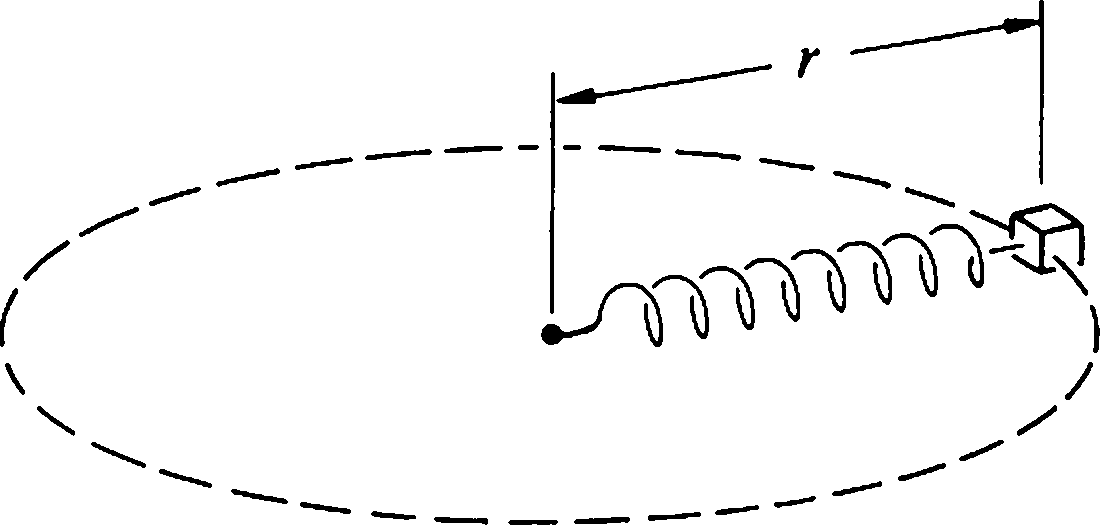
\includegraphics[width=0.33\textwidth]{ps10_1}\end{center}
  \begin{enumerate}[(a)]
    \item Find the radius of the orbit and the velocity of the body.
    \item The body is struck by a sudden sharp blow, giving it instantaneous velocity of 1 m / s radially outward. Show the state of the system before and after the blow on a sketch of the energy diagram.
    \item For the new orbit, find the maximum and minimum values of $r$.
  \end{enumerate}
\section{Problem \thesection: K\&K 9.7}
  A rocket is in an elliptic orbit around the earth. To put it in escape orbit, its engine is briefly fired, changing the rocket's velocity by $\Delta \vec v$. Where in the orbit, and in what direction, should the firing occur to attain escape with a minimum value of $\Delta \vec v$?
\section{Problem \thesection: K\&K 9.9}
  Halley's comet is in an elliptic orbit about the sun. The eccentricity of the orbit is $\varepsilon = 0.967$ and the period is $T = 76$ y. The mass of the sun is $m_s = 1.99 \cdot 10^{30}$ kg.  The mass of Halley's comet is negligible compared to the sun.
  \begin{enumerate}[(a)]
    \item Using this data, determine the distance of Halley's comet at closest approach to the sun, perihelion, and furthest distance from the sun, aphelion.
    \item What is the speed of Halley's comet when it is closest to the sun?
  \end{enumerate}
\section{Problem \thesection: K\&K 9.10}
  A satellite of mass $m_s$ is in a circular orbit about the earth. The radius of the orbit is $r_0$ and the mass of the earth is $m_e$.
  \begin{enumerate}[(a)]
    \item Find the total mechanical energy of the satellite.
    \item Now suppose that the satellite moves in the extreme upper atmosphere of the earth where it is retarded by a constant feeble friction force $f$. The satellite will spiral slowly to the earth. Since the friction force is weak, the change in radius will be very slow. We can therefore assume that at any given instant the satellite is in a circular orbit of average radius $r$. Find the approximate change in radius per revolution of the satellite, $\Delta r$.
    \item Find the approximate change in kinetic energy per revolution of the satellite, $\Delta K$.
  \end{enumerate}
\section{Problem \thesection: K\&K 9.12}
  A space vehicle is in a circular orbit about the earth. The mass of the vehicle is $m_s = 3.00 \cdot 10^3$ kg and the radius of the orbit is $2R_e = 1.28 \cdot 10^4$ km. It is desired to transfer the vehicle to a circular orbit of radius $4R_e$.
  \begin{center}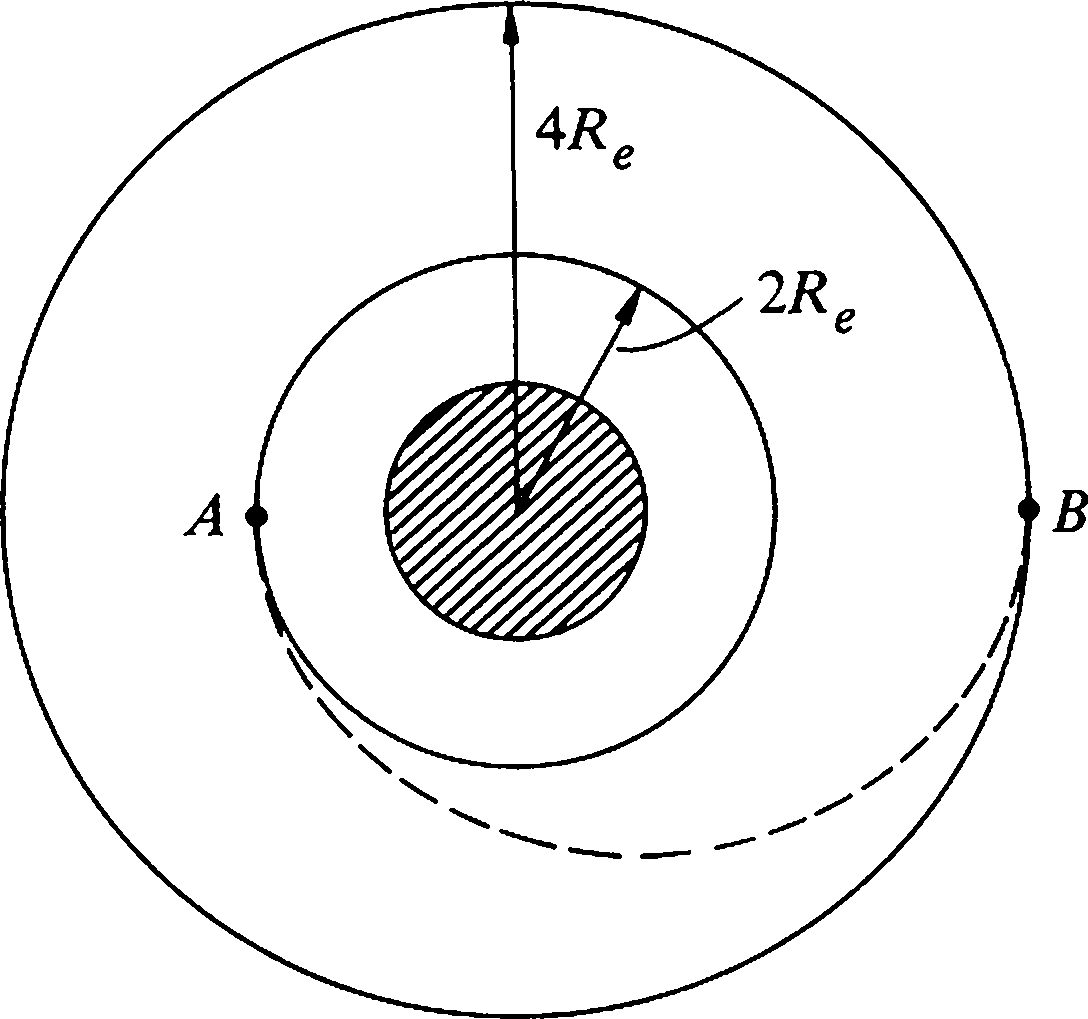
\includegraphics[width=0.33\textwidth]{ps10_2}\end{center}
  \begin{enumerate}[(a)]
    \item What is the minimum energy expenditure required for the transfer?
    \item An efficient way to accomplish the transfer is to use a semielliptical orbit from point $A$ from the inner circular orbit at to point $B$ at the outer circular orbit (known as a Hohmann transfer orbit). What velocity changes are required at the points of intersection, $A$ and $B$?
  \end{enumerate}
\section{Problem \thesection: The Motion of SO-2 around the Black Hole at the Galactic Center}
  \subsection{Background}
    The UCLA Galactic Center Group, headed by Dr. Andrea Ghez, reported the following data, (see \url{http://www.astro.ucla.edu/\~ghezgroup/gc/} for information about the research group, and \url{http://www.astro.ucla.edu/\~ghezgroup/gc/images/2004orbit_animfull_sm.gif} for an animation of the orbits about the galactic center), for the orbits of eight stars within $0.8'' \times 0.8''$ of the galactic center.
    \begin{center}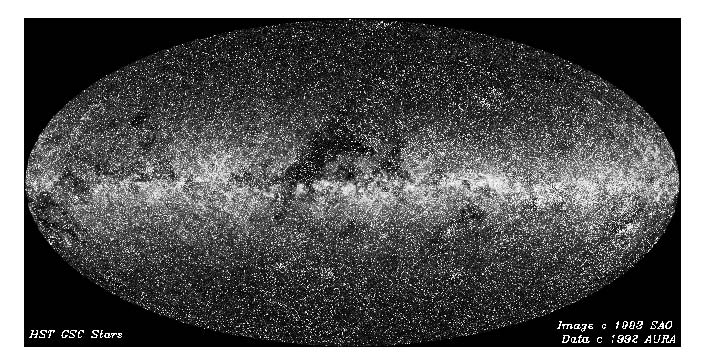
\includegraphics[width=0.75\textwidth]{ps10_3}\end{center}
    The orbits of the stars are shown in \hyperref[fig:orbits]{Figure 1}.

    \begin{figure}[!h] \label{fig:orbits}
      \begin{center}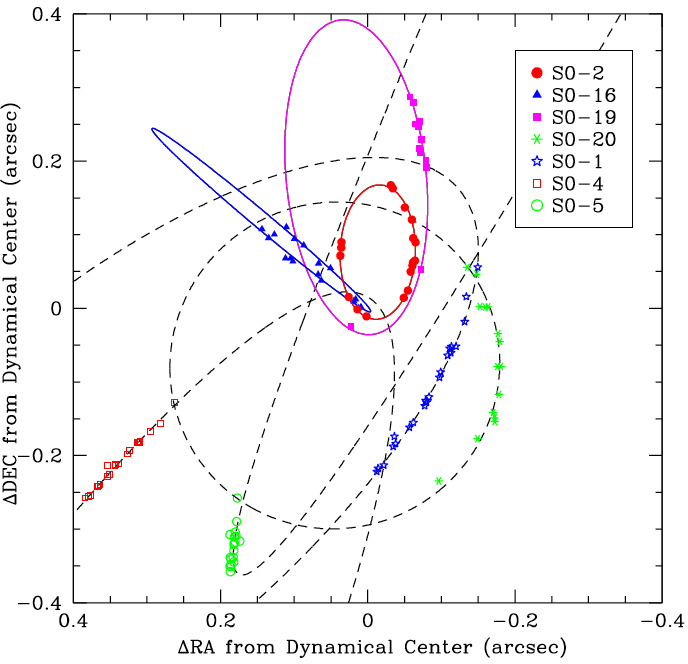
\includegraphics[width=0.75\textwidth]{ps10_4}\end{center}
    \end{figure}
    \refstepcounter{figure}

    A standard astronomical unit is the parsec. One parsec is the distance at which there is one arcsecond = 1/3600 deg angular separation between two objects that are separated by the distance of one astronomical unit, 1 AU${} = 1.50 \cdot 10^{11}$ m which is the mean distance between the earth and sun. One astronomical unit is roughly equivalent to eight light minutes,  1 AU${} = 8.3$ lmin.  One parsec is equal to 3.26 light years, where one light year is the distance that light travels in one earth year, 1 pc${} = {}$3.26 ly${} = 2.06 \cdot 10^5$ AU where 1 ly${} = 9.46 \cdot 10^{15}$ m. The orbital data for the star SO-2, S0-16, and S0-19 are as follows\footnote{A.M.Ghez, et al., Stellar Orbits Around Galactic Center Black Hole, preprint arXiv:astro-ph/0306130v1, 5 June, 2003.}:
    \begin{center}
      \begin{tabular}{|l|l|l|l|l|l|}
        \hline Star  & Period          & Eccentricity  & Semi-major axis     & Periapse (AU) & Apoapse (AU) \\
                     & (yrs)           &               & ($10^{-3}$ arc sec) &               &              \\
        \hline S0-2  & 15.2            & 0.8763        & 120.7 (4.5)         & 119.5 (3.9)   & 1812 (73)    \\
                     & (0.68 / 0.76)   & (0.0063)      &                     &               &              \\
        \hline S0-16 & 29.9 (6.8 / 13) & 0.943 (0.019) & 191 (24)            & 87 (17)       & 2970 (560)   \\
        \hline S0-19 & 71 (35 / 11000) & 0.889 (0.065) & 340 (220)           & 301 (41)      & 5100 (3600)  \\ \hline
      \end{tabular}
    \end{center}
    The period of S0-2 satisfies Kepler's Third Law given by
    $$T^2 = \frac{4\pi^2 a^3}{G(m_1 + m_2)}$$
    where $m_1$ is the mass of S0-2, $m_2$ is the mass of the black hole, and a is the semi-major axis of the elliptic orbit of S0-2.

    The orbit data is given in terms of properties of the elliptic orbit. Consider the ellipse shown in the figure below.
    \begin{figure}[!h]
      \begin{center}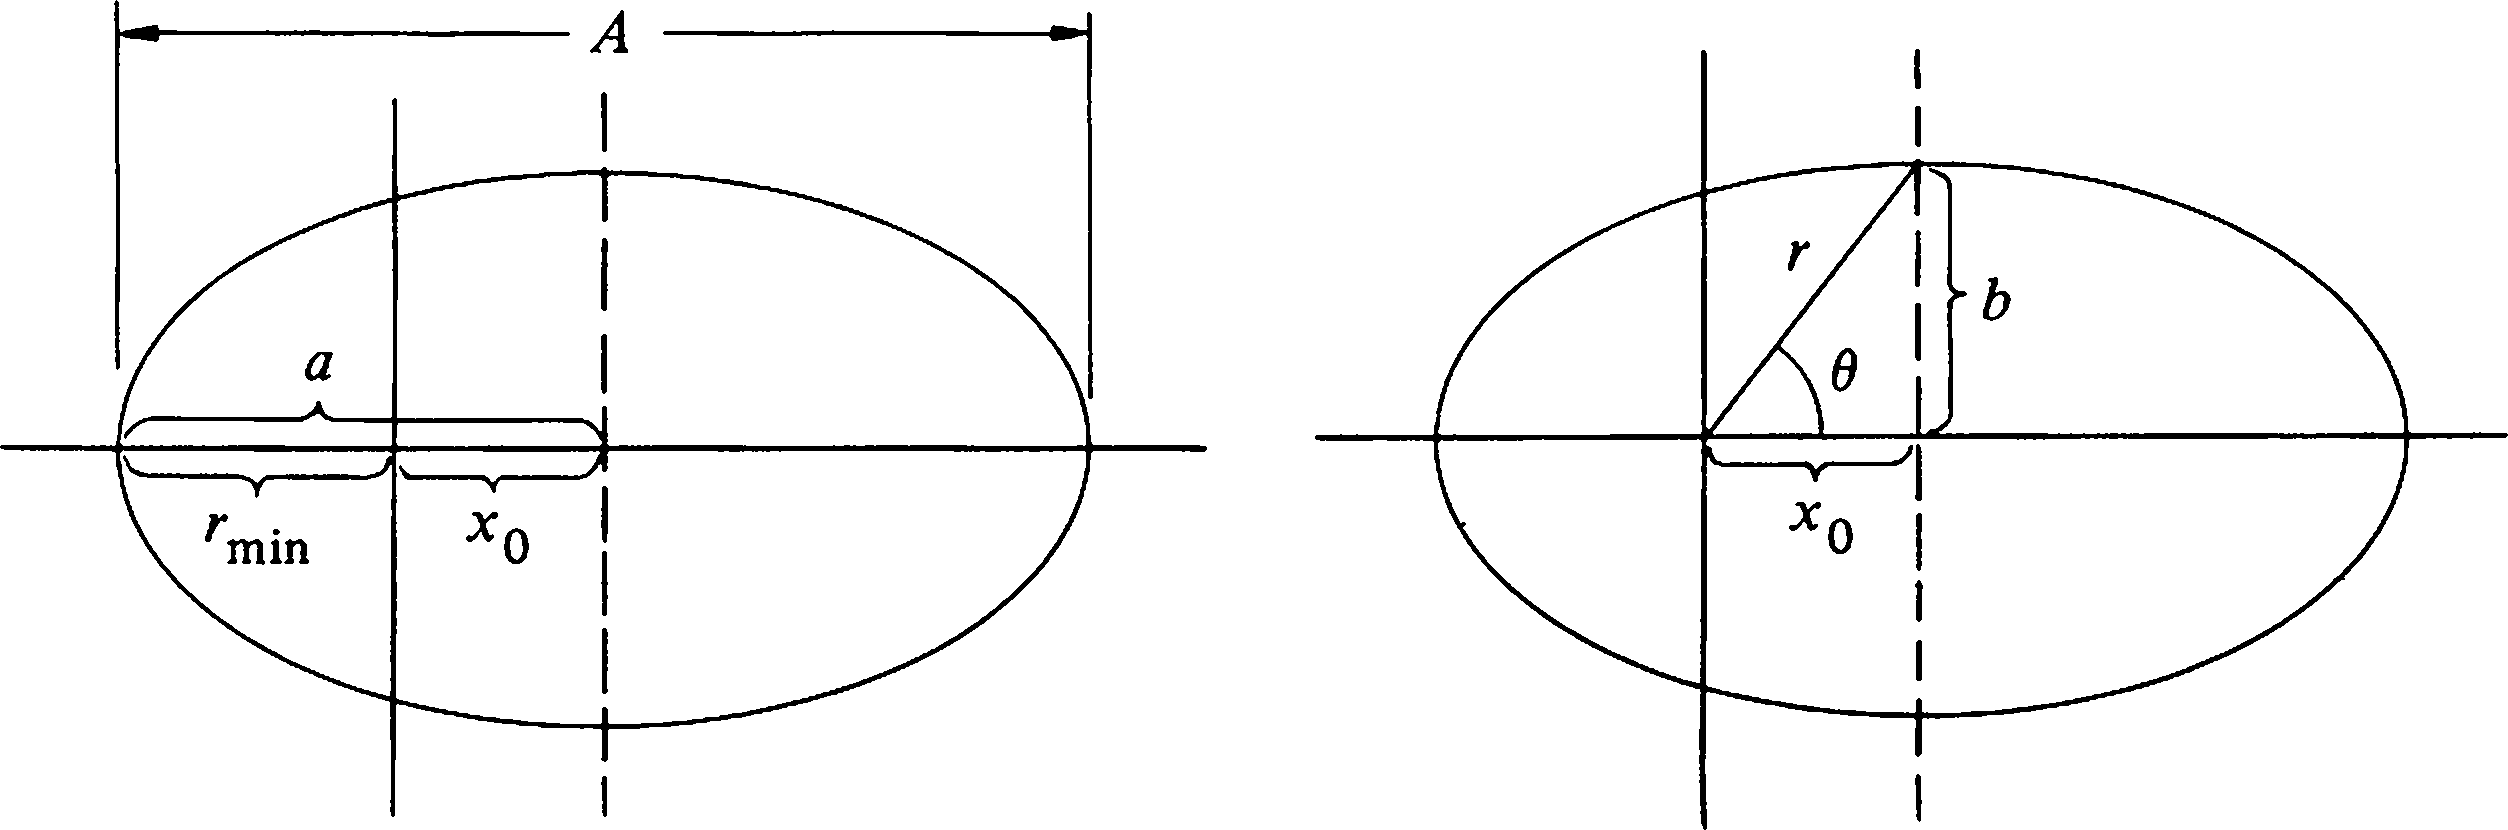
\includegraphics[width=0.6\textwidth]{ps10_5}\end{center}
      \caption{elliptic orbit} \label{fig:ellipse}
    \end{figure}
    In \autoref{fig:ellipse}, let $a$ denote the semi-major axis, $b$ denote the semi-minor axis, and $x_0$ denote the location of the center of the ellipse from one focal point $P$.

    The orbit equation for the system is given by
    $$r = \frac{r_0}{1 - \varepsilon\cos\theta},$$
    where $r_0$ and the eccentricity $\varepsilon$ are two constants.

    The constant $r_0$ can be found by considering the lowest energy circular orbit which has radius
    $$r_0 = \frac{L^2}{\mu G m_1 m_2,}$$
    where $\mu = \frac{m_1 m_2}{m_1 + m_2}$ is the reduced mass. Note that S0-2 is in a much higher energy orbit.

    The energy of this circular orbit is
    $$E_0 = -\frac{G m_1 m_2}{2r_0}.$$
    The eccentricity of the elliptic orbit of S0-2 is then
    $$\varepsilon = (1 - E / E_0)^{1/2} = \left(1 + \frac{2 E L^2}{\mu(G m_1 m_2)^2}\right)^{1/2}$$
    The semi major axis $a$ is given by
    $$a = \frac{r_p + r_a}{2}$$
    where the distance of furthest approach is denoted by $r_a$, and is called apoapse for the orbit about the galactic center), and the distance of nearest approach is denoted by $r_p$, and is called periapse for the orbit about the galactic center.
    \begin{figure}[!h]
      \begin{center}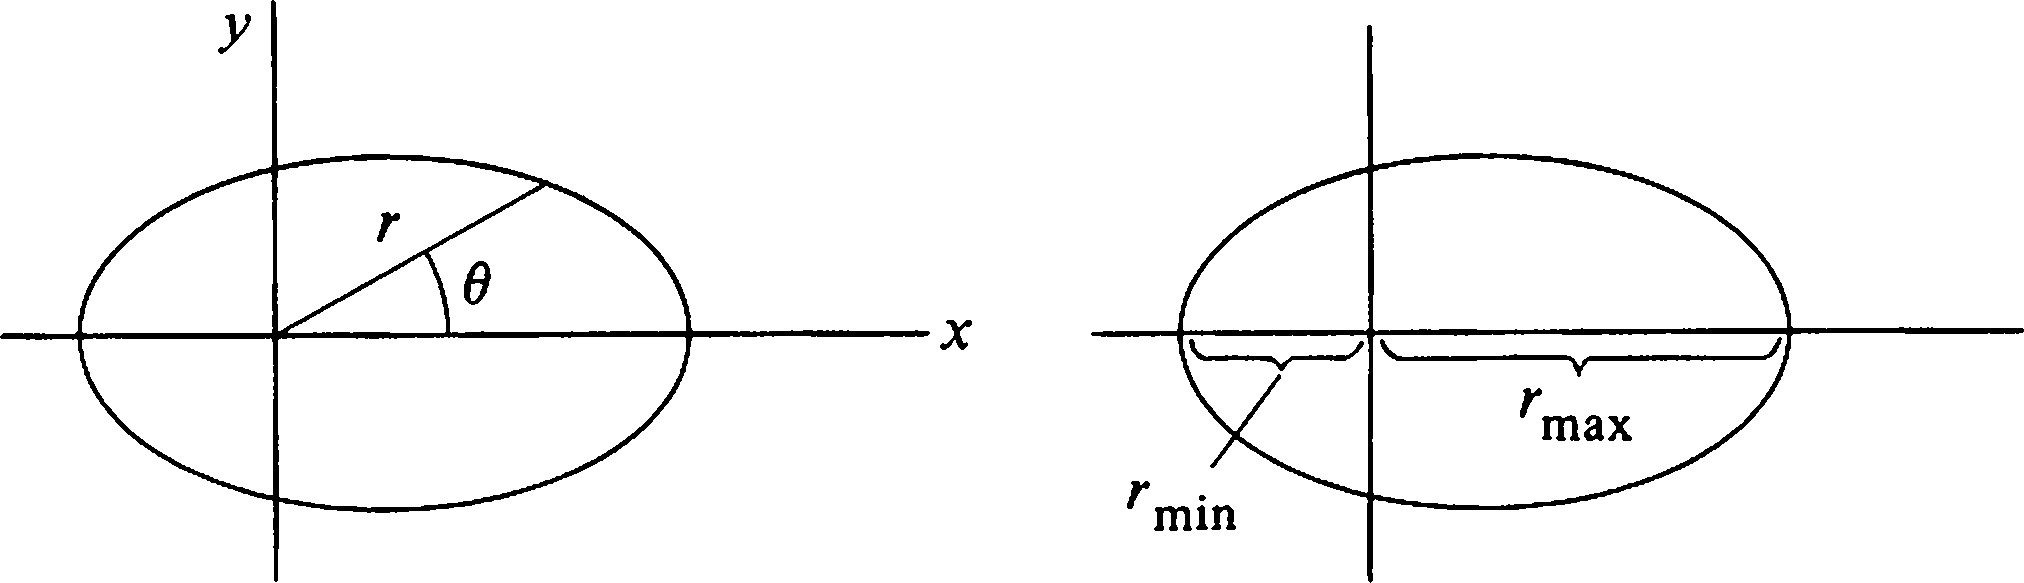
\includegraphics[width=0.75\textwidth]{ps10_6}\end{center}
      \caption{Nearest and furthest approach}
    \end{figure}

  \subsection{Questions:}
    \begin{enumerate}[(a)]
      \item Using the results in the data table for the star S0-2, find the length of the semimajor axis.
      \item Using the results in the data table for the star S0-2, find the mass of the black hole that the star S0-2 is orbiting. How many solar masses does this correspond to?  Use $G = 6.67 \cdot 10^{-11}$ N m$^2$ kg$^{-2}$ and the mass of the sun is given by $m_s = 1.99 \cdot 10^{30}$ kg.
      \item Use the equations for constant energy and angular momentum to find the velocity at periapse and apoapse.
      \item Assume that the S0-2 orbit is perpendicular to our line of sight. With this assumption, how far away is S0-2 from the earth?
    \end{enumerate}
\end{document}
